\documentclass{article}
% Some basic packagesLLuu
\usepackage[utf8]{inputenc}
\usepackage{spverbatim}
\usepackage[margin=1.2in]{geometry}
\usepackage{textcomp}
\usepackage{url}
\usepackage{graphicx}
\usepackage{float}
\usepackage{algorithm2e}
% \usepackage{algorithm}
\usepackage{enumitem}
\usepackage{standalone}
\usepackage{tcolorbox}
\usepackage{wrapfig}
% \usepackage{svg}
% \usepackage{svg-inkscape} 

\graphicspath{{./figures}}


%color settings
\usepackage{xcolor}
% \definecolor{gruvbgdark}{HTML}{1d2021}
% \definecolor{gruvtextdark}{HTML}{ebdbb2}
% \definecolor{gruvbglight}{HTML}{f9f5d7}
% \definecolor{gruvtextlight}{HTML}{3c3836}
% \definecolor{NavyBlue}{HTML}{266bbd}
% \definecolor{RawSienna}{HTML}{94330e}
% \definecolor{ForestGreen}{HTML}{149b52}
% \pagecolor{gruvbgdark}
% \color{gruvtextdark}

\definecolor{GBBlue}{HTML}{458588}
\definecolor{GBGreen}{HTML}{98971A}
\definecolor{GBRed}{HTML}{CC241D}
\definecolor{GBYellow}{HTML}{D79921}
\definecolor{GBPurple}{HTML}{B16286}
\definecolor{GBAqua}{HTML}{689D6A}
\definecolor{GBOrange}{HTML}{D65D0E}
\definecolor{GBGray}{HTML}{A89984}
\definecolor{GBDarkGray}{HTML}{3C3836}
\definecolor{GBLightGray}{HTML}{EBDBB2}
\definecolor{GBBackground}{HTML}{282828}
\definecolor{GBForeground}{HTML}{FBF1C7}
\pagecolor{GBBackground}
\color{GBForeground}
% Hide page number when page is empty
\usepackage{emptypage}
\usepackage{subcaption}
\usepackage{multicol}

% Math stuff
\usepackage{amsmath, amsfonts, mathtools, amsthm, amssymb}
% Fancy script capitals
\usepackage{mathrsfs}
\usepackage{cancel}

% Bold math
\usepackage{bm}

%Algorithm setup
\RestyleAlgo{algoruled}
% Some shortcuts
\newcommand\N{\ensuremath{\mathbb{N}}}
\newcommand\R{\ensuremath{\mathbb{R}}}
\newcommand\Z{\ensuremath{\mathbb{Z}}}
\renewcommand\O{\ensuremath{\emptyset}}
\newcommand\Q{\ensuremath{\mathbb{Q}}}
\newcommand\C{\ensuremath{\mathbb{C}}}
\newcommand\B{\ensuremath{\mathbb{B}}}

%Make implies and impliedby shorter
\let\implies\Rightarrow
\let\impliedby\Leftarrow
\let\iff\Leftrightarrow


% Add \contra symbol to denote contradiction
% \usepackage{stmaryrd} % for \lightning
% \newcommand\contra{\scalebox{1.5}{$\lightning$}}

\let\phi\varphi

% Command for short corrections
% Usage: 1+1=\correct{3}{2}

\definecolor{correct}{HTML}{009900}
\newcommand\correct[2]{\ensuremath{\:}{\color{red}{#1}}\ensuremath{\to }{\color{correct}{#2}}\ensuremath{\:}}
\newcommand\green[1]{{\color{correct}{#1}}}

% horizontal rule
% \newcommand\hr{
%     \noindent\rule[0.5ex]{\linewidth}{0.5pt}
% }

% hide parts
\newcommand\hide[1]{}

% Environments
\makeatother

% For box around Definition, Theorem, \ldots
% theorems
\usepackage{thmtools}
\usepackage[framemethod=TikZ]{mdframed}
\mdfsetup{skipabove=1em,skipbelow=1em, innertopmargin=5pt, innerbottommargin=6pt}

\theoremstyle{definition}

\makeatletter

\declaretheoremstyle[headfont=\bfseries, bodyfont=\normalfont, numbered=no]{idea}

\declaretheoremstyle[
	headfont=\bfseries\color{ForestGreen!70!black}, bodyfont=\normalfont,
    postheadspace=\newline,
	mdframed={
			linewidth=2pt,
			rightline=false, topline=false, bottomline=false,
			linecolor=ForestGreen, backgroundcolor=ForestGreen!5,
		},
    numberwithin=section
]{thmgreenbox}

\declaretheoremstyle[
	headfont=\bfseries\color{NavyBlue!70!black}, bodyfont=\normalfont,
    postheadspace=\newline,
	mdframed={
			linewidth=2pt,
			rightline=false, topline=false, bottomline=false,
			linecolor=NavyBlue, backgroundcolor=NavyBlue!5,
		},
    numberwithin=section
]{thmbluebox}
\declaretheoremstyle[
	headfont=\bfseries\color{NavyBlue!70!black}, bodyfont=\normalfont,
	mdframed={
			linewidth=2pt,
			rightline=false, topline=false, bottomline=false,
			linecolor=NavyBlue, backgroundcolor=NavyBlue!5,
		},
    numberwithin=section
]{thmclaimbox}

\declaretheoremstyle[
	headfont=\bfseries\color{NavyBlue!70!black}, bodyfont=\normalfont,
	mdframed={
			linewidth=2pt,
			rightline=false, topline=false, bottomline=false,
			linecolor=NavyBlue
		},
    numberwithin=section
]{thmblueline}

\declaretheoremstyle[
	headfont=\bfseries\color{RawSienna!70!black}, bodyfont=\normalfont,
    postheadspace=\newline,
	mdframed={
			linewidth=2pt,
			rightline=false, topline=false, bottomline=false,
			linecolor=RawSienna, backgroundcolor=RawSienna!5,
		},
    numberwithin=section
]{thmredbox}

\declaretheoremstyle[
	headfont=\bfseries\color{RawSienna!70!black}, bodyfont=\normalfont,
    postheadspace=\newline,
	mdframed={
			linewidth=2pt,
			rightline=false, topline=false, bottomline=false,
			linecolor=RawSienna, backgroundcolor=RawSienna!5,
		},
	qed=\qedsymbol,
    numberwithin=section
]{thmproofbox}

\declaretheoremstyle[
	headfont=\bfseries\color{NavyBlue!70!black}, bodyfont=\normalfont,
	numbered=no,
	mdframed={
			linewidth=2pt,
			rightline=false, topline=false, bottomline=false,
			linecolor=NavyBlue, backgroundcolor=NavyBlue!1,
		},
]{thmexplanationbox}

\declaretheorem[style=thmgreenbox, name=Definition]{definition}
\declaretheorem[style=thmbluebox, numbered=no, name=Problem Statement]{stmt}
\declaretheorem[style=thmbluebox, numbered=no, name=Answer]{ans}
\declaretheorem[sibling=definition, style=thmredbox, name=Corollary]{corollary}
\declaretheorem[style=thmbluebox, numbered=no, name=Idea]{idea}
\declaretheorem[style=thmbluebox,  name=Proposition]{prop}
\declaretheorem[style=thmredbox, name=Theorem]{theorem}
\declaretheorem[style=thmproofbox, name=Proof]{prf}
\declaretheorem[style=thmredbox, name=Lemma]{lemma}
\declaretheorem[style=thmclaimbox, numbered=no, name=Claim]{claim}
\declaretheorem[numbered=no, style=thmexplanationbox, name=Proof]{explanation}
\declaretheorem[numbered=no, style=thmproofbox, name=Proof]{replacementproof}
\declaretheorem[style=thmgreenbox,  numbered=no, name=Task]{ex}
\declaretheorem[style=thmbluebox,  numbered=no, name=Example]{eg}
\declaretheorem[style=thmblueline, numbered=no, name=Remark]{remark}
\declaretheorem[style=thmblueline, numbered=no, name=Note]{note}

\renewenvironment{proof}[1][\proofname]{\begin{replacementproof}}{\end{replacementproof}}
\AtEndEnvironment{eg}{\null\hfill$\diamond$}%

\newtheorem*{uovt}{UOVT}
\newtheorem*{notation}{Notation}
\newtheorem*{previouslyseen}{As previously seen}
\newtheorem*{problem}{Problem}
\newtheorem*{observe}{Observe}
\newtheorem*{property}{Property}
\newtheorem*{intuition}{Intuition}

\newcommand{\oefening}[1]{%
	\def\@oefening{#1}%
	\subsection*{Oefening #1}
}

\newcommand{\suboefening}[1]{%
	\subsubsection*{Oefening \@oefening.#1}
}


% \lecture starts a new lecture (les in dutch)
%
% Usage:
% \lecture{1}{di 12 feb 2019 16:00}{Inleiding}
%
% This adds a section heading with the number / title of the lecture and a
% margin paragraph with the date.

% I use \dateparts here to hide the year (2019). This way, I can easily parse
% the date of each lecture unambiguously while still having a human-friendly
% short format printed to the pdf.

% \usepackage{xifthen}
% \def\testdateparts#1{\dateparts#1\relax}
% \def\dateparts#1 #2 #3 #4 #5\relax{
% 	\marginpar{\small\textsf{\mbox{#1 #2 #3 #5}}}
% }

% \def\@lecture{}%
% \newcommand{\lecture}[3]{
% 	\ifthenelse{\isempty{#3}}{%
% 		\def\@lecture{Lecture #1}%
% 	}{%
% 		\def\@lecture{Lecture #1: #3}%
% 	}%
% 	\subsection*{\@lecture}
% 	% \marginpar{\small\textsf{\mbox{#2}}}
% }

\usepackage{listings}

\definecolor{dkgreen}{rgb}{0,0.6,0}
\definecolor{gray}{rgb}{0.5,0.5,0.5}
\definecolor{mauve}{rgb}{0.58,0,0.82}

\lstset{frame=single,
  language=c,
  aboveskip=3mm,
  belowskip=3mm,
  showstringspaces=false,
  columns=flexible,
  basicstyle={\small\ttfamily},
  numbers=none,
  numberstyle=\tiny\color{GBForeground},
  keywordstyle=\color{GBRed},
  commentstyle=\color{GBGreen},
  stringstyle=\color{GBAqua},
  breaklines=true,
  breakatwhitespace=true,
  tabsize=2
}



% These are the fancy headers
\usepackage{fancyhdr}
\pagestyle{fancy}

% LE: left even
% RO: right odd
% CE, CO: center even, center odd
% My name for when I print my lecture notes to use for an open book exam.
\fancyhead[LE,RO]{Kristian Sørdal}

\fancyhead[RO,LE]{INF236 - Parallel Programmering} % Right odd,  Left even
% \fancyhead[RE,LO]{\leftmark}          % Right even, Left odd
\fancyhead[RE,LO]{Kristian Sørdal}          % Right even, Left odd

% \fancyfoot[RO,LE]{\thepage}  % Right odd,  Left even
% \fancyfoot[RE,LO]{Kristian Sørdal}          % Right even, Left odd
% \fancyfoot[C]{\leftmark}     % Center

\makeatother

% Todonotes and inline notes in fancy boxes
\usepackage{todonotes}
\usepackage{tcolorbox}

% Make boxes breakable
\tcbuselibrary{breakable}

% Figure support as explained in my blog post.
\usepackage{import}
\usepackage{xifthen}
\usepackage{pdfpages}
\usepackage{transparent}
\newcommand{\incfig}[2][1]{%
	% \begin{center}
	\def\svgwidth{#1\columnwidth}
	\import{./figures/}{#2.pdf_tex}
	% \end{center}
}
% Fix some stuff
% %http://tex.stackexchange.com/questions/76273/multiple-pdfs-with-page-group-included-in-a-single-page-warning
\pdfsuppresswarningpagegroup=1
\author{Kristian Sørdal}

\usepackage{pgfplots}
\pgfplotsset{compat=1.17}


\title{INF236 - Assignment 1}

\begin{document}
\maketitle
\newpage
\tableofcontents
\newpage
    
    \section*{Problem 1}
    \addcontentsline{toc}{section}{Problem 1}

    The implementation of sequential radix sort has been implemented in the following manner.

\begin{algorithm}[H]
    \caption{Sequential Radix Sort}
    \SetKwInOut{Input}{Input}
    \SetKwInOut{Output}{Output}
    \SetAlgoVlined
    \SetKwFor{For}{for}{do}{}
    \SetKw{KwTo}{to}
    \SetKw{KwBy}{by}
    
    \Input{\(n\) - The length of the array, \(b\) - Key size (how many bits to interpret as one digit)}
    \Output{\(t\) - the time taken to sort the array}
    \(a \leftarrow\) array of random unsigned 64-bit integers of size \(n\)

    \(tmp \leftarrow\) partially sorted array of size \(n\), initialized with 0

    \(buckets \gets 2^{b}\)
    
    \For{\(shift \gets 0\) \KwTo \(64\) \KwBy \(b\)}{
        \(bucketSize \leftarrow\) array of size \(buckets\), initialized with 0
        
        \For{\(i \gets 0\) \KwTo \(n - 1\)}{
            \(bucket \gets (a[i] \gg shift) \& (buckets - 1)\)

            \(bucketSize[bucket]\)++
        }
        
        % verify this is correct
        \(sum \gets 0\)\;

        \( bucketSize[0] \gets 0 \)

        \For{\(i \gets 1\) \KwTo \(buckets - 1\)}{
            % \(sum \gets sum + bucketSize[i]\)
            \( t \gets sum  + bs[i] \)

            \(bucketSize[i] \gets t\)

            \( sum \gets t \)
        }
        
        \For{\(i \gets 0\) \KwTo \(n-1\)}{
            \(bucket \gets (a[i] \gg shift) \& (buckets - 1)\)

            \(tmp[bucketSize[bucket]\)\(] \gets a[i]\)

            \( bucketSize[bucket] \)++
        }
        

        % for (int i = 0; i < n; i++) {
        %     ull val = a[i];                         // get value
        %     int t = (val >> shift) & (buckets - 1); // get bucket
        %     permuted[bs[t]++] = val;
        % }
        \(a \gets tmp\)\;
    }
\end{algorithm}

Firstly, we allocate memory for \( a \) and \( tmp \). \( a \) represents the input array, and will also contain the final sorted array, whereas \( tmp \) will store the partially sorted array during execution. \( a \) will be swapped with \( tmp \) every time the outermost for loop is done executing one iteration.
\medskip

The outermost for loop iterates from 0 to 64, with a step size of \( b \), where \( b \) represents how many bits should be interpreted as one digit. It iterates up to 64 bits, as this is the size of an \texttt{unsigned long long} type in \texttt{c}.
\medskip

Each time this for loop iterates, it goes through 3 stages.

\paragraph{Stage 1 - Counting how many elements for each bucket}
In this stage, we iterate through the array containing our values. For each element \( x \) stored in \( a[i] \), we want to figure out in which bucket this element should be placed into. Given \( s \), representing the power we should raise \( x \) to, and \( k \), representing how many buckets there are, we can obtain \( b \), representing the bucket \( x \) belongs in. This can be done with the following formula

\[ b = \left\lfloor\frac{x}{2^{s}}\right\rfloor \wedge k-1 \]

Which can be implemented in \texttt{c} as \(bucket \leftarrow (a[i] \gg shift) \& (buckets - 1)\).

\paragraph{Stage 2 - Prefix sum}
In this stage, we need to perform a prefix sum operation on the \( bucketSize \) array. This is done in order to ensure we start placing the elements in the buckets at the correct index in the \( tmp \) array in the next stage.

\paragraph{Stage 3 - Creating the partially sorted array}
In this stage, we need to place our elements at the correct index in the \( tmp \) array. This is done by again, computing which bucket element \( a[i] \) belongs to. After we have found the bucket, we place this element in the \( tmp \) array, at index \( bucketSize[bucket] \). Because we performed the prefix sum over the \( bucketSize \) array in the previous stage, this variable contains the index at which the elements belonging to this bucket should be placed in the \( tmp \) array. After we have placed element \( a[i] \), we increment this index pointer, such that we avoid overwriting anything.


\section*{Problem 2}
\addcontentsline{toc}{section}{Problem 2}

Through trial and error, the maximum elements that could be sorted in 10 seconds, was 52 million, with a value of \( b = 4 \). Varying \( b \) by powers of 2, we obtain the following execution times for sorting 52 million elements



\begin{figure}[H]
    \begin{center}
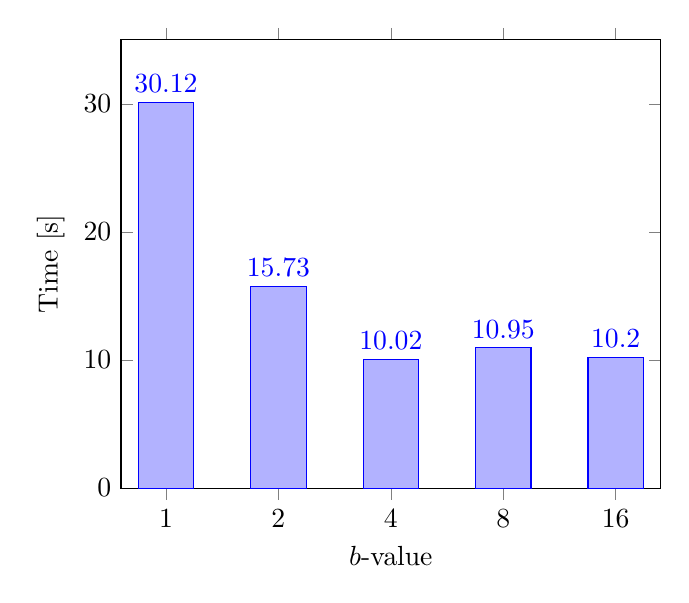
\begin{tikzpicture}
\begin{axis}[
    ybar,
    ymin=0,
    ymax=35,
    ylabel={Time [s]},
    xmode=log, % Set the x-axis to logarithmic mode
    log basis x={2}, % Base for the logarithm (optional, default is 10)
    xtick={1,2,4,8,16}, % Specify tick positions
    log ticks with fixed point, % Display ticks as fixed point numbers
    xlabel={\( b \)-value},
    bar width=20pt,
    xticklabel=\pgfmathparse{2^\tick}\pgfmathprintnumber{\pgfmathresult}, % Convert log ticks back to normal numbers
    nodes near coords,
]
% Add the data, ensuring the x values are in the log scale (if necessary)
\addplot coordinates {(1,30.116869) (2,15.729472) (4,10.024868) (8,10.947608) (16,10.204863)};
\end{axis}
\end{tikzpicture}
    \end{center}
    \caption{Sorting 52 million elements with varying \( b \) values}
\end{figure}

    % So in order to compute an equation \( T\left( n,b \right) \) which yields the time the sequential program takes to run, we need to consider the amount of FLOPS the sequential program uses, and the clock speed of the CPU on Brake.
\end{document}
